\documentclass[letterpaper,11pt]{article}
\pdfoutput=1

% packages
\usepackage{mathtools}
\usepackage{amssymb}
\usepackage{braket}
\usepackage{mathrsfs}
\usepackage{tikz}
\usepackage{subfig}
\usepackage{xspace}
\usepackage{xcolor}
\usepackage{float}
\usepackage{color}
\usepackage{siunitx}
\usepackage{comment}
\usepackage{afterpage}
\usepackage{multirow}
\usepackage{array}
\usepackage{hhline}
\usepackage{amsthm}
\usepackage{framed}
\usepackage[utf8]{inputenc}
\usepackage[countmax]{subfloat}
\usepackage{fullpage}
\usepackage{pdfpages}
\usepackage{amsfonts}
\usepackage{blindtext}
\usepackage{hyperref}
\usepackage{cite}

\def\PZ{Z\xspace}
\def\PW{W\xspace}
\def\PQt{t\xspace}
\def\PAQt{\bar{t}\xspace}
\def\PQq{q\xspace}
\def\cPgn{\nu\xspace}
\def\Pl{\ell}
\def\jet{j}

\def\ttZ{t$\bar{\text{t}}$Z\xspace}
\def\ttG{t$\bar{\text{t}}\gamma$\xspace}
\def\ttW{t$\bar{\text{t}}$W\xspace}
\def\ttbar{t$\bar{\text{t}}$\xspace}
\def\WZ{WZ\xspace}
\def\tZq{tZq\xspace}
\def\tWZ{tWZ\xspace}

\def\pT{p$_\text{T}$}
\def\pTZ{p$_\text{T}$(Z)\xspace}
\def\cosThetaStar{$\cos\theta^*_\text{Z}$\xspace}
\def\nlep{N$_\text{lep}$\xspace}

\def\ctZ{C$_\text{tZ}$\xspace}
\def\ctZI{C$_\text{tZ}^\text{[Im]}$\xspace}
\def\cpt{C$_{\phi \text{t}}$\xspace}
\def\cpQM{C$_{\phi \text{Q}}$\xspace}

\def\delphes{\texttt{Delphes}\xspace}
\def\MGvATNLO{\texttt{MADGRAPH5aMC@NLO}\xspace}
\def\PYTHIA{\texttt{PYTHIA}\xspace}
\def\MadSpin{\texttt{MadSpin}\xspace}

\def\TeV{TeV\xspace}
\def\GeV{GeV\xspace}

\title{Anomalous couplings in the tt+Z final state at the HL-LHC}
\author{Lukas Lechner, Daniel Spitzbart, Robert Sch\"ofbeck}
\date{}

\begin{document}

\maketitle

\section{Introduction}\label{sec:introduction}

Many beyond the Standard Model (BSM) predictions include anomalous couplings of the top quark to the electroweak gauge bosons~\cite{Hollik:1998vz,Agashe:2006wa,Kagan:2009bn,Ibrahim:2010hv,Ibrahim:2011im,Grojean:2013qca,Richard:2013pwa}.
While we restrict this study to the \ttZ channel and the CMS Phase-2 detector with a luminosity scenario of 3~ab${}^{-1}$, we go beyond earlier work~\cite{Rontsch:2015una} and study the sensitivity of the \ttZ process using differential cross section data.
We interpret the result in terms of the SM effective field theory~\cite{AguilarSaavedra:2018nen} and set limits on the relevant Wilson coefficients of the Warsaw basis~\cite{Grzadkowski:2010es} \ctZ, \ctZI, \cpt and \cpQM~\cite{Brehmer:2016nyr, Brehmer:2017fyp}.

\section{Event simulation}
\label{sec:eventsimulation}
We generate events at the parton level at LO using \MGvATNLO~v2.3.3~\cite{Alwall:2014hca}, and decay them using \MadSpin~\cite{Artoisenet:2012st, Frixione:2007zp}.
Parton showering and hadronization are done using \PYTHIA 8.2~\cite{Sjostrand:2007gs,Sjostrand:2014zea}.
Fast detector simulation was performed using \delphes~\cite{deFavereau:2013fsa}, with the CMS reconstruction efficiency parametrization for the Phase-2 upgrade.
The mean number of interactions per bunch crossing (pileup, PU) is varied from 0 to 200.
Jets are reconstructed with the {\texttt FastJet} package~\cite{Cacciari:2011ma} and using the anti-$k_T$ algorithm~\cite{Cacciari:2008gp} with a cone size $R=0.4$.
Besides the signals, we also generate the main backgrounds in the leptonic final states in order to achieve a realistic background prediction.
The \WZ, \tZq, \tWZ, \ttG and \ttZ processes are normalized to cross sections calculated up to next-to-leading order (NLO) in perturbative QCD.

\section{Event selection}
\label{sec:selection}
From results on the inclusive \ttZ cross section from ATLAS~\cite{Aad:2015eua,ATLAS:2016ttVarticles} and CMS~\cite{PRL-110-172002,EPJC-C74-2014-9,JHEP-1601-2016-096,Sirunyan:2017uzs} it follows that the three lepton channel, where the \PZ and one of the \PW~bosons originating from a top~quark decay leptonically is the most sensitive search channel.
We thus require three reconstructed leptons (e~or~$\mu$) with \pT($\Pl$) thresholds of 10, 20, and 40~\GeV, respectively, and $|\eta(\Pl)|<3.0$.
We furthermore require that there is among them a pair of opposite-sign same-flavor leptons consistent with the \PZ~boson by requiring $|m(\Pl\Pl)-m_\text{\PZ}|<10$~\GeV.
We remove reconstructed leptons within a cone of $\Delta R < 0.3$ to any reconstructed jet satisfying \pT(\jet) $>$ 30~\GeV.
Furthermore, at least 3 jets are required with \pT(\jet) $>$ 30~\GeV and $|\eta($\jet$)|<4.0$, where one of the jets has been identified as a b-tag jet according to the \delphes specification.

\noindent
We consider the distributions of the observables above in equally sized bins of the transverse \PZ~boson momenta \pTZ~\cite{Rontsch:2014cca} and \cosThetaStar, the relative angle of the negatively charged lepton to the \PZ~boson direction of flight in the rest frame of the boson.
The differential cross sections for the SM (black) and BSM (colored lines) interpretations in \ttZ with respect to \pTZ and \cosThetaStar are shown in Fig.~\ref{fig:ttZ_pt_cos} for \ctZ = 2~($\Lambda$/\TeV)$^2$ and \ctZI = 2~($\Lambda$/\TeV)$^2$.
We normalize the BSM distributions to the SM yield in the plots to visualize the discriminating features of the parameters.
The part of the signal which does not contain information on the Wilson coefficients is shown hatched, backgrounds are shown in solid colors.

\begin{figure}[tbp]
  \centering
    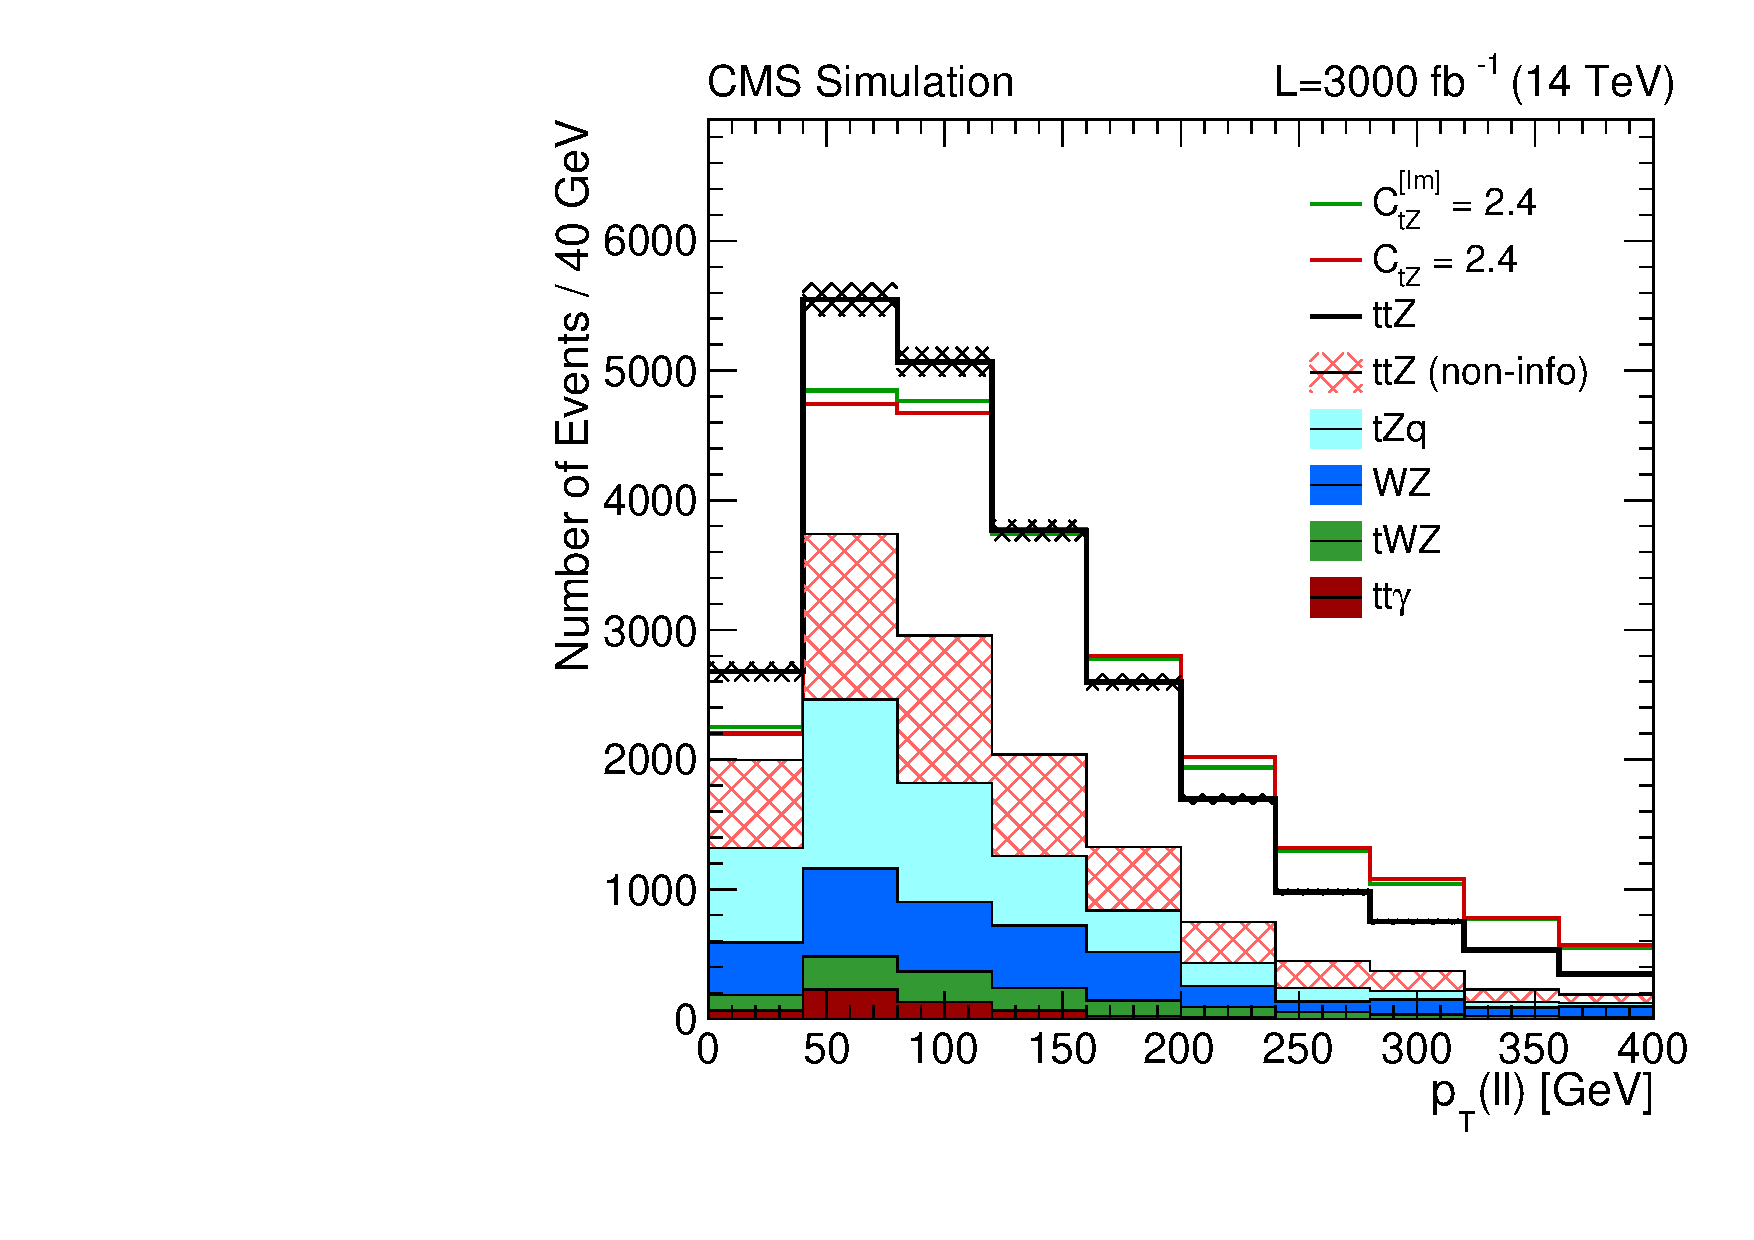
\includegraphics[trim={0.2cm 1.cm 0.4cm 0.cm},clip,width=0.40\textwidth]{Figures/Z_pt_lin.pdf}
    \hspace{1.7cm}
    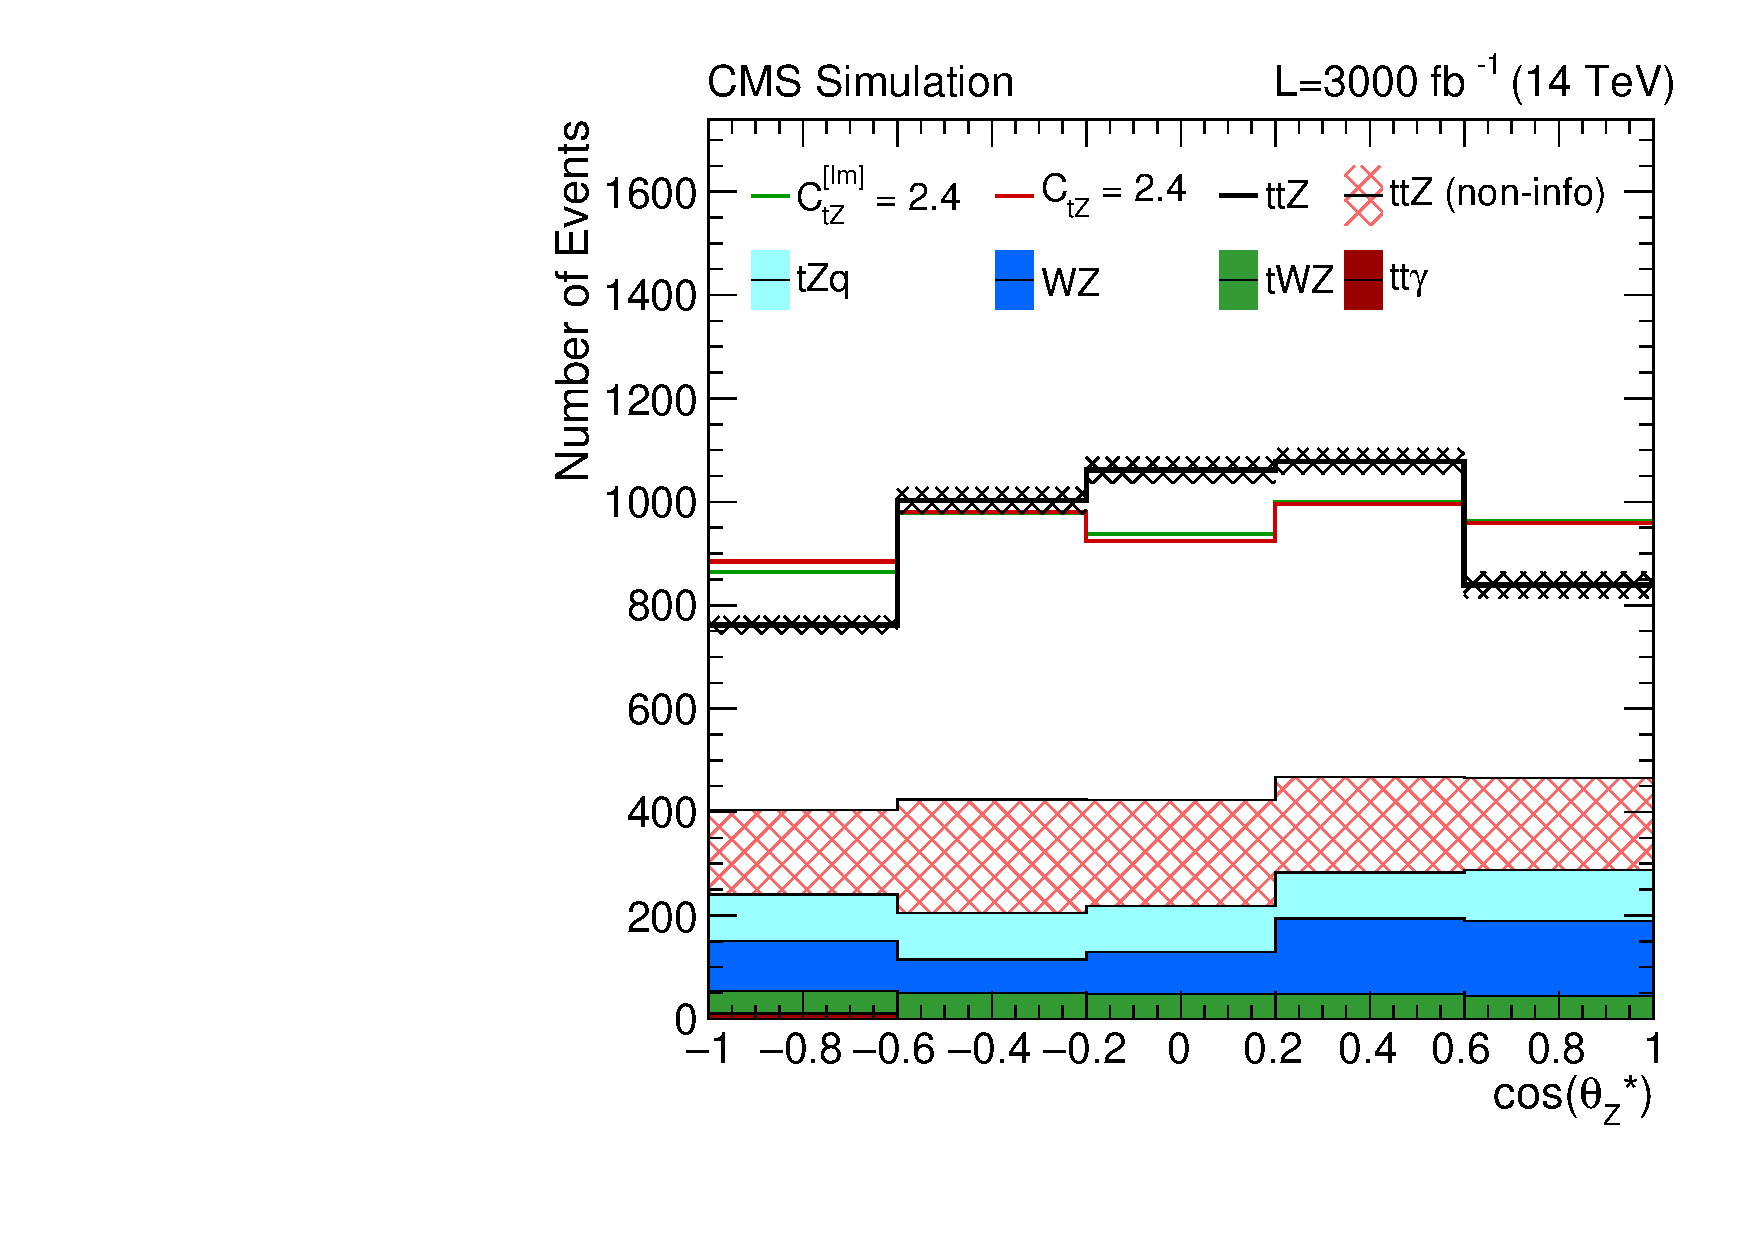
\includegraphics[trim={0.2cm 1.cm 0.4cm 0.cm},clip,width=0.40\textwidth]{Figures/Z_costheta_lin_ptZ200.pdf}
    \hspace{.3cm}
\caption{
Differential cross sections of \pTZ (left) and \cosThetaStar (right) for the in the text mentioned selection and the Phase-2 scenario.
For \cosThetaStar, additionally \pTZ $>$ 200~\GeV is applied. 
}\label{fig:ttZ_pt_cos}
\end{figure}

\section{Results}
\label{sec:results}

The predicted yields are estimated for the 3~ab${}^{-1}$ HL-LHC scenario at $\sqrt{s}=13$~\TeV and scaled to 14~\TeV, where an additional small background from non-prompt leptons is taken from Ref.~\cite{Sirunyan:2017uzs} and scaled to 3~ab${}^{-1}$.
We perform a profiled maximum likelihood fit of the binned likelihood function $L(\theta)$ and consider $q(r)=-2\log(L(\hat{\theta})/L(\hat{\theta}_{\textrm{SM}}))$, where $\hat{\theta}$ and
$\hat{\theta}_\textrm{SM}$ are the set of nuisance parameters maximizing $L(\theta)$ at the BSM and SM point, respectively.
Experimental uncertainties are estimated based on the expected performance of the Phase-2 CMS detector.
In Fig.~\ref{fig:ttZ_1Dnll}, the likelihood scan for the \ttZ process is shown, where we consider one non-zero Wilson coefficient at a time, and all others are set to zero.
The corresponding 68\% and 95\% CL intervals are summarized in Table~\ref{tab:limits}.
In Fig.~\ref{fig:ttZ_1Dprofnll}, likelihood ratios for two pairs of Wilson coefficients corresponding to modified neutral current interactions (\cpt and \cpQM) and dipole moment interactions (\ctZ and \ctZI) are considered.
The Wilson coefficient not shown on the $x$ axis is included in the profiling of nuisance parameters.
The corresponding 68\% and 95\% CL intervals are summarized in Table~\ref{tab:proflimits}.
In Fig.~\ref{fig:ttZ_nll}, the log-likelihood scan for the \ttZ process is shown in the \cpQM/\cpt parameter plane~(left) and the dipole moment parameter plane \ctZ/\ctZI~(right).
The green (red) lines show the 68\% (95\%) CL contour line and the SM parameter point corresponds to \cpt = \cpQM = 0 and \ctZ = \ctZI = 0.


\begin{table}[h]
\caption{Expected 68~\% and 95~\% CL intervals, where one Wilson coefficient at a time is considered non-zero.}\label{tab:limits}
\begin{center}
\begin{tabular}{c|c|c}
\hline
Wilson coefficient & 68~\% CL $(\Lambda/$TeV$)^2$ & 95~\% CL $(\Lambda/$TeV$)^2$ \\
\hline
\hline
\cpt   & [-0.47, 0.47]                 & [-0.89, 0.89]                 \\
\hline
\cpQM  & [-0.38, 0.38]                 & [-0.75, 0.73]                 \\
\hline
\ctZ   & [-0.37, 0.36]                 & [-0.52, 0.51]                 \\
\hline
\ctZI  & [-0.38, 0.36]                 & [-0.54, 0.51]                 \\
\hline
\end{tabular}
\end{center}
\end{table}

\begin{table}[h]
\caption{Expected 68~\% and 95~\% CL intervals for the selected Wilson coefficients in a profiled scan over the 2D parameter planes \cpQM/\cpt and \ctZ/\ctZI. The respective second parameter of the scan is left free.}\label{tab:proflimits}
\begin{center}
\begin{tabular}{c|c|c}
\hline
Wilson coefficient & 68~\% CL $(\Lambda/$TeV$)^2$ & 95~\% CL $(\Lambda/$TeV$)^2$ \\
\hline
\hline
\cpt   & [-1.65, 3.37]                 & [-2.89, 6.76]                 \\
\hline
\cpQM  & [-1.35, 2.92]                 & [-2.33, 6.69]                 \\
\hline
\ctZ   & [-0.37, 0.36]                 & [-0.52, 0.51]                 \\
\hline
\ctZI  & [-0.38, 0.36]                 & [-0.54, 0.51]                 \\
\hline
\end{tabular}
\end{center}
\end{table}

\begin{figure}[tbp]
  \centering
    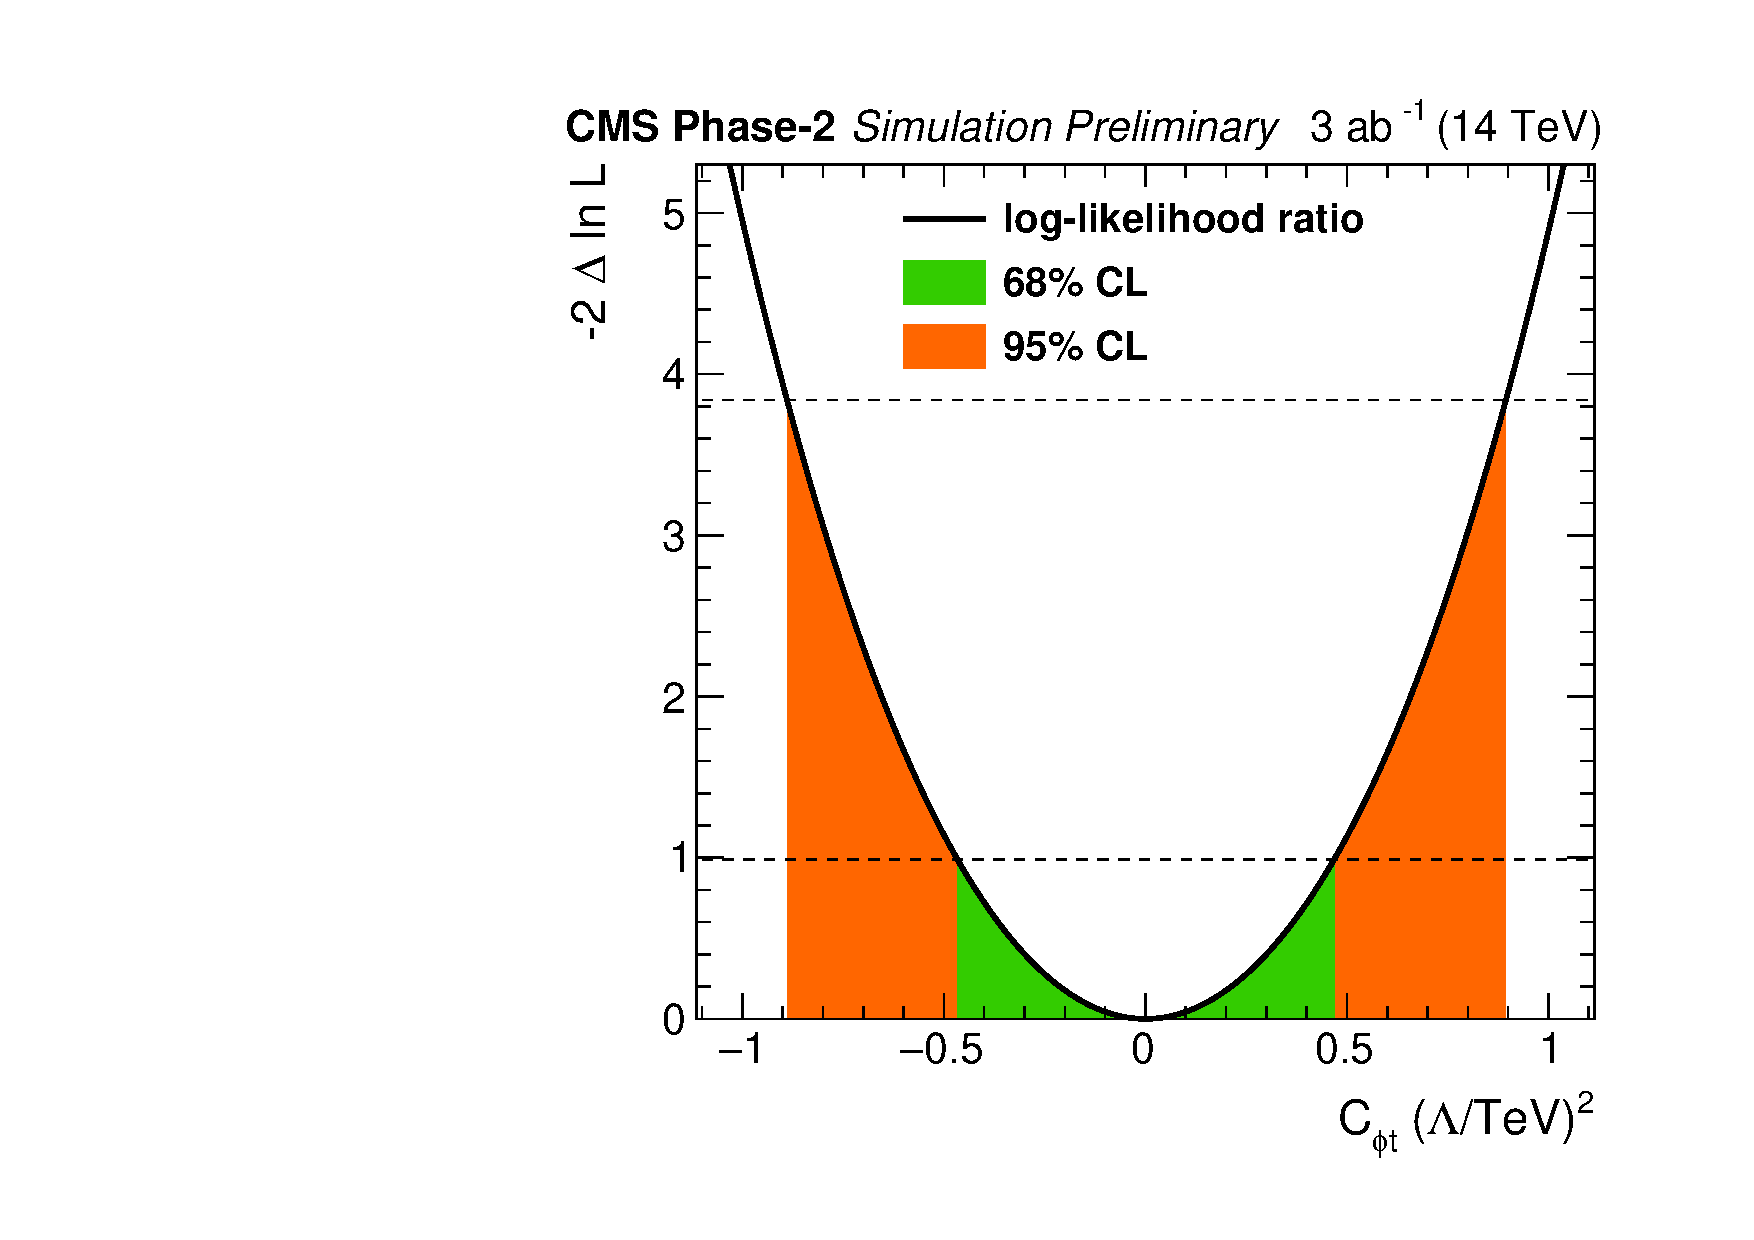
\includegraphics[trim={0.4cm 0.cm 0.8cm 0.cm},clip,width=0.45\textwidth]{Figures/1D_cpt_lumi3000_14TeV_CMScombine_r1_fullUnc.pdf}
    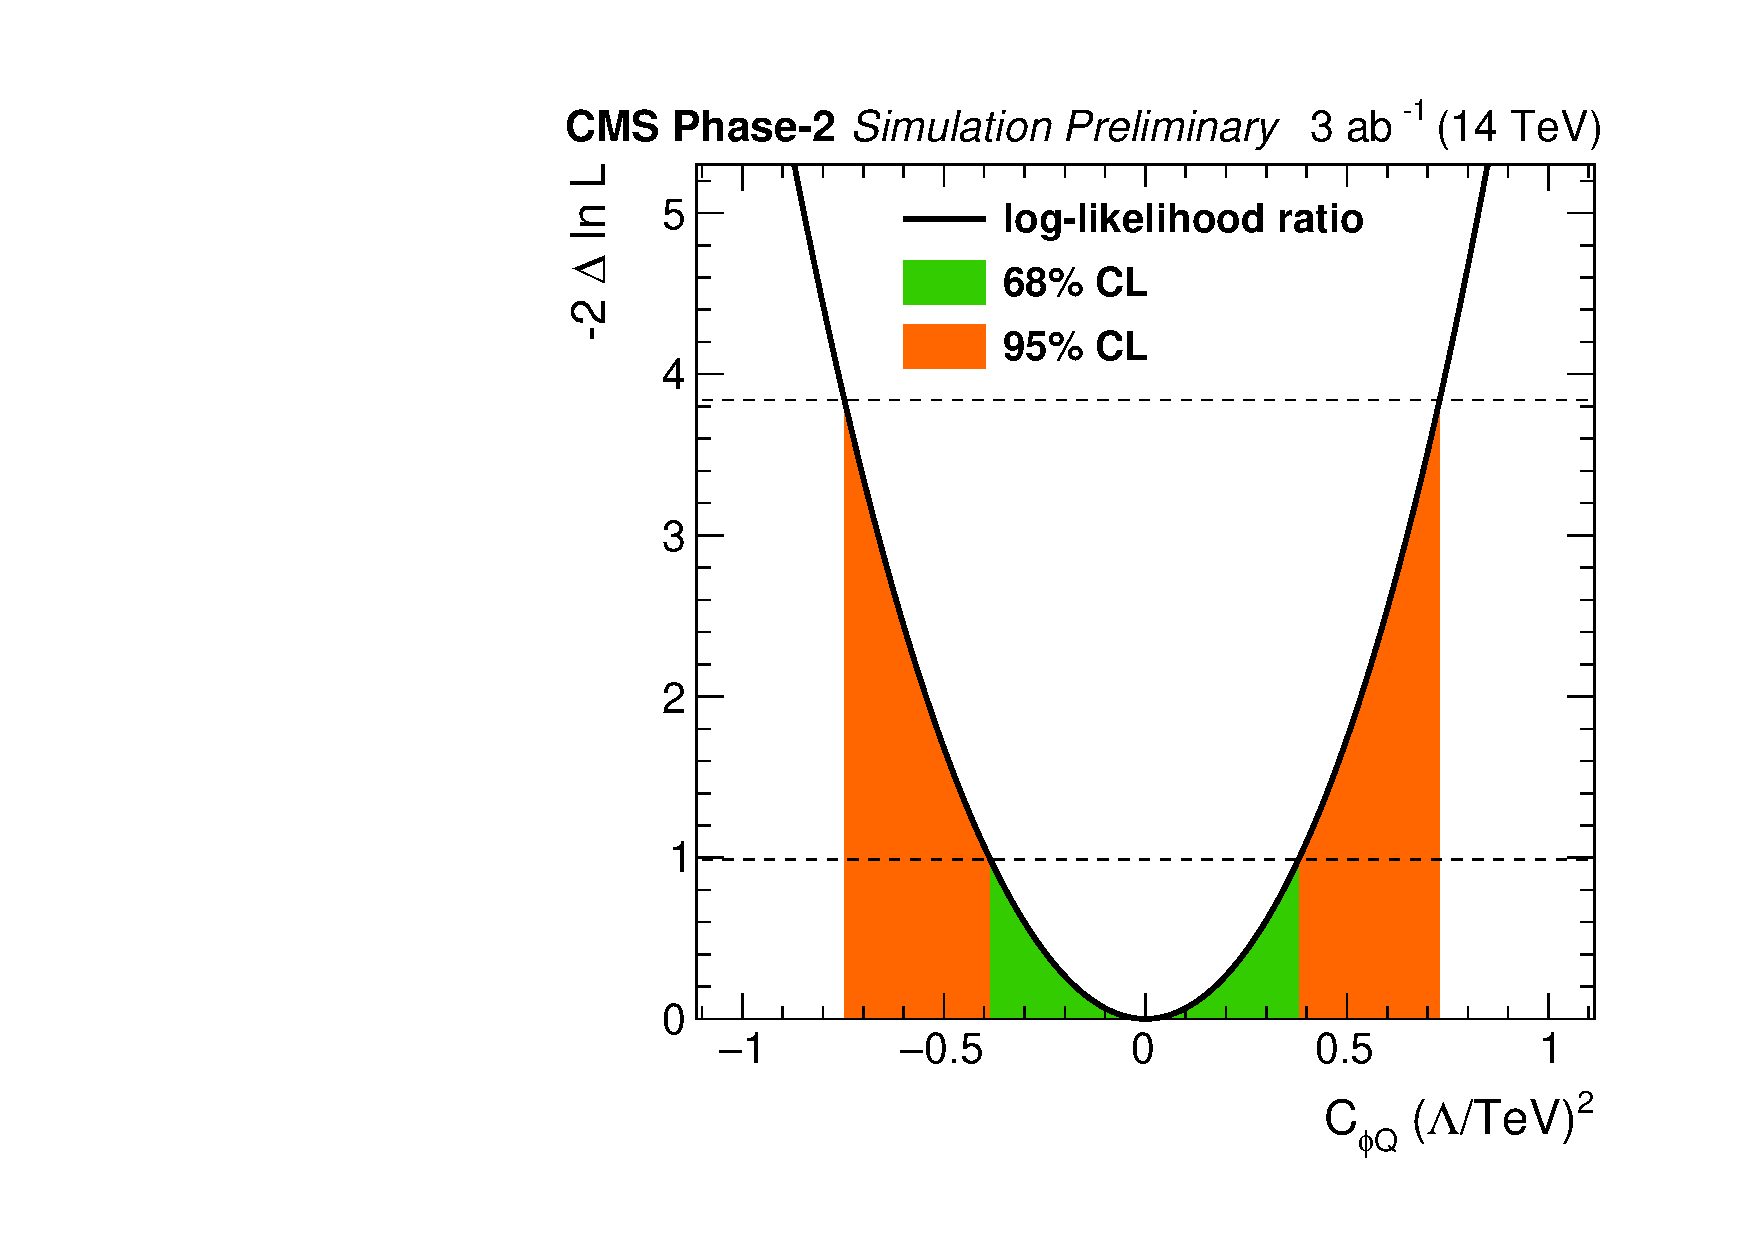
\includegraphics[trim={0.4cm 0.cm 0.8cm 0.cm},clip,width=0.45\textwidth]{Figures/1D_cpQM_lumi3000_14TeV_CMScombine_r1_fullUnc.pdf}
    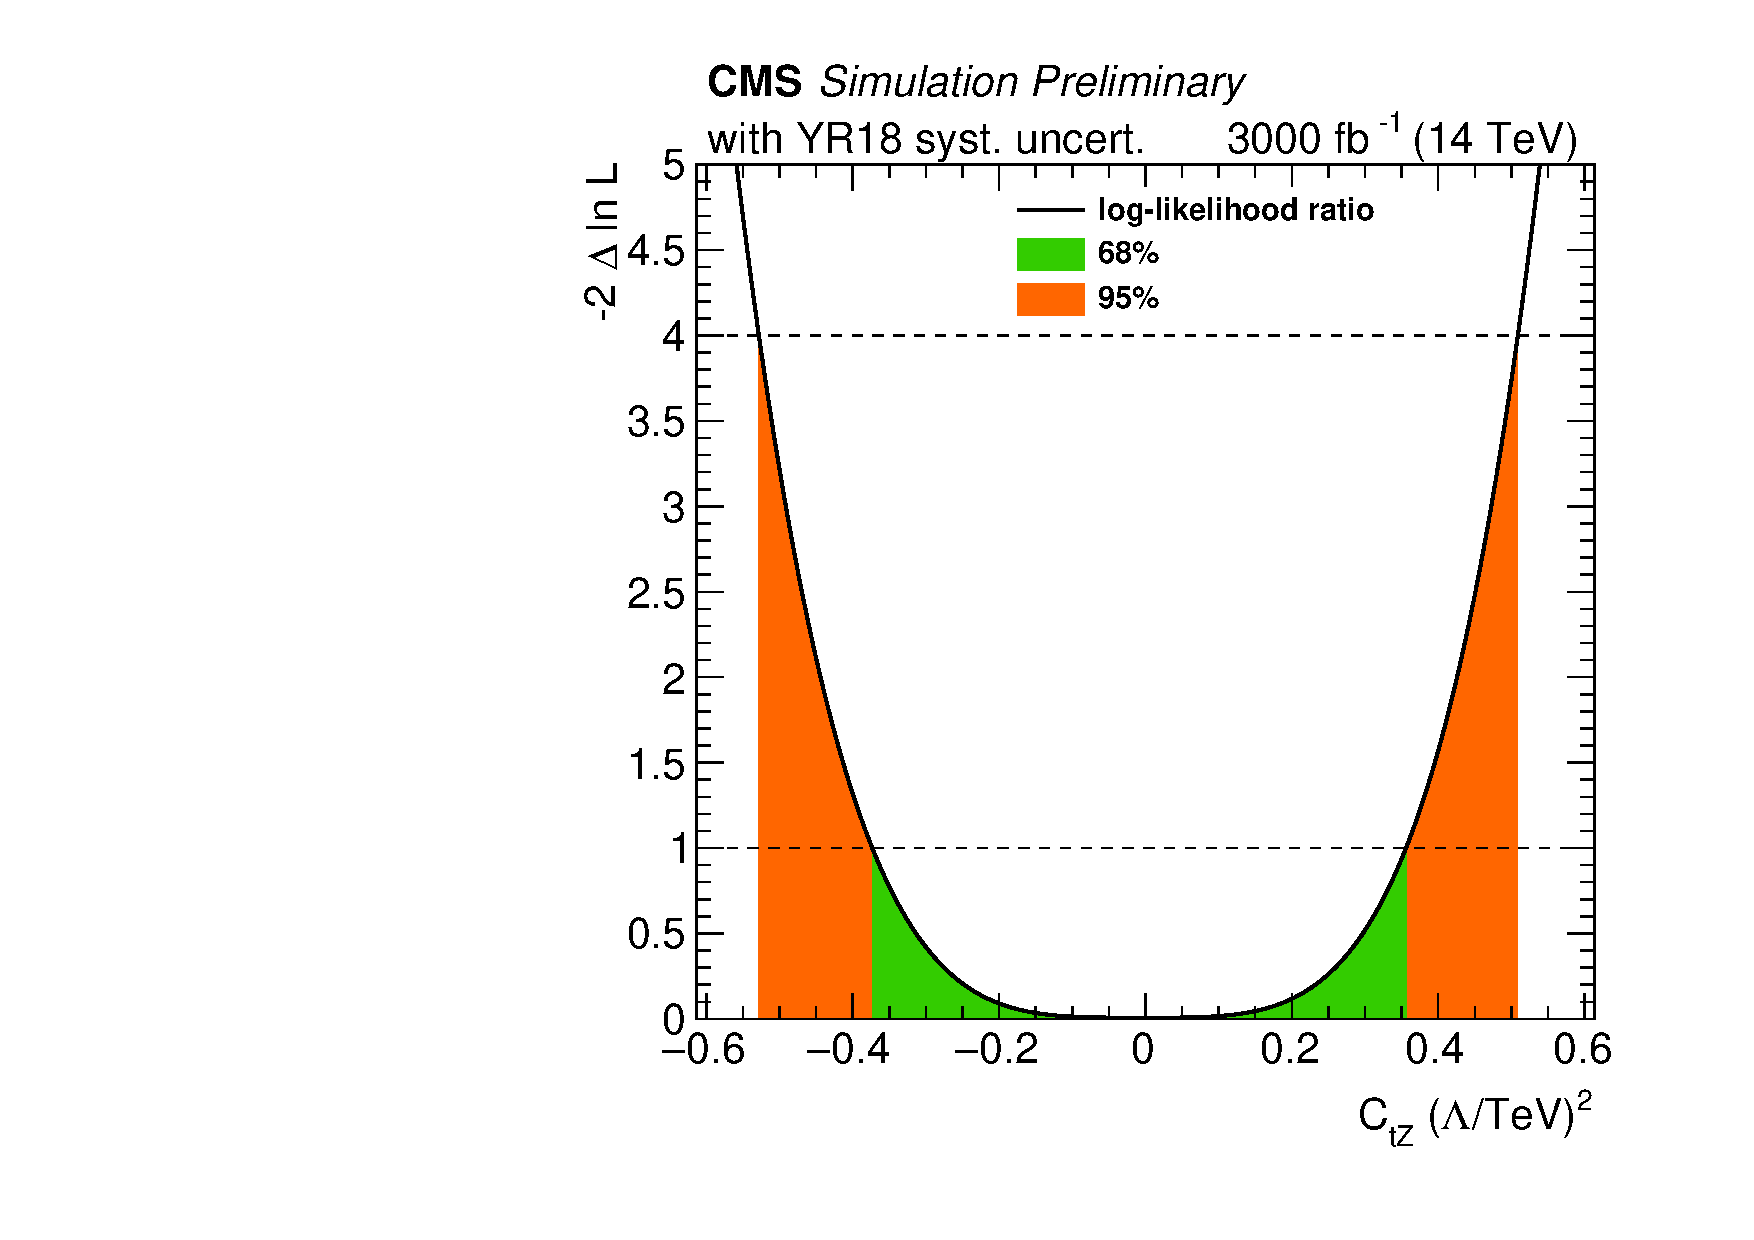
\includegraphics[trim={0.4cm 0.cm 0.8cm 0.cm},clip,width=0.45\textwidth]{Figures/1D_ctZ_lumi3000_14TeV_CMScombine_r1_fullUnc.pdf}
    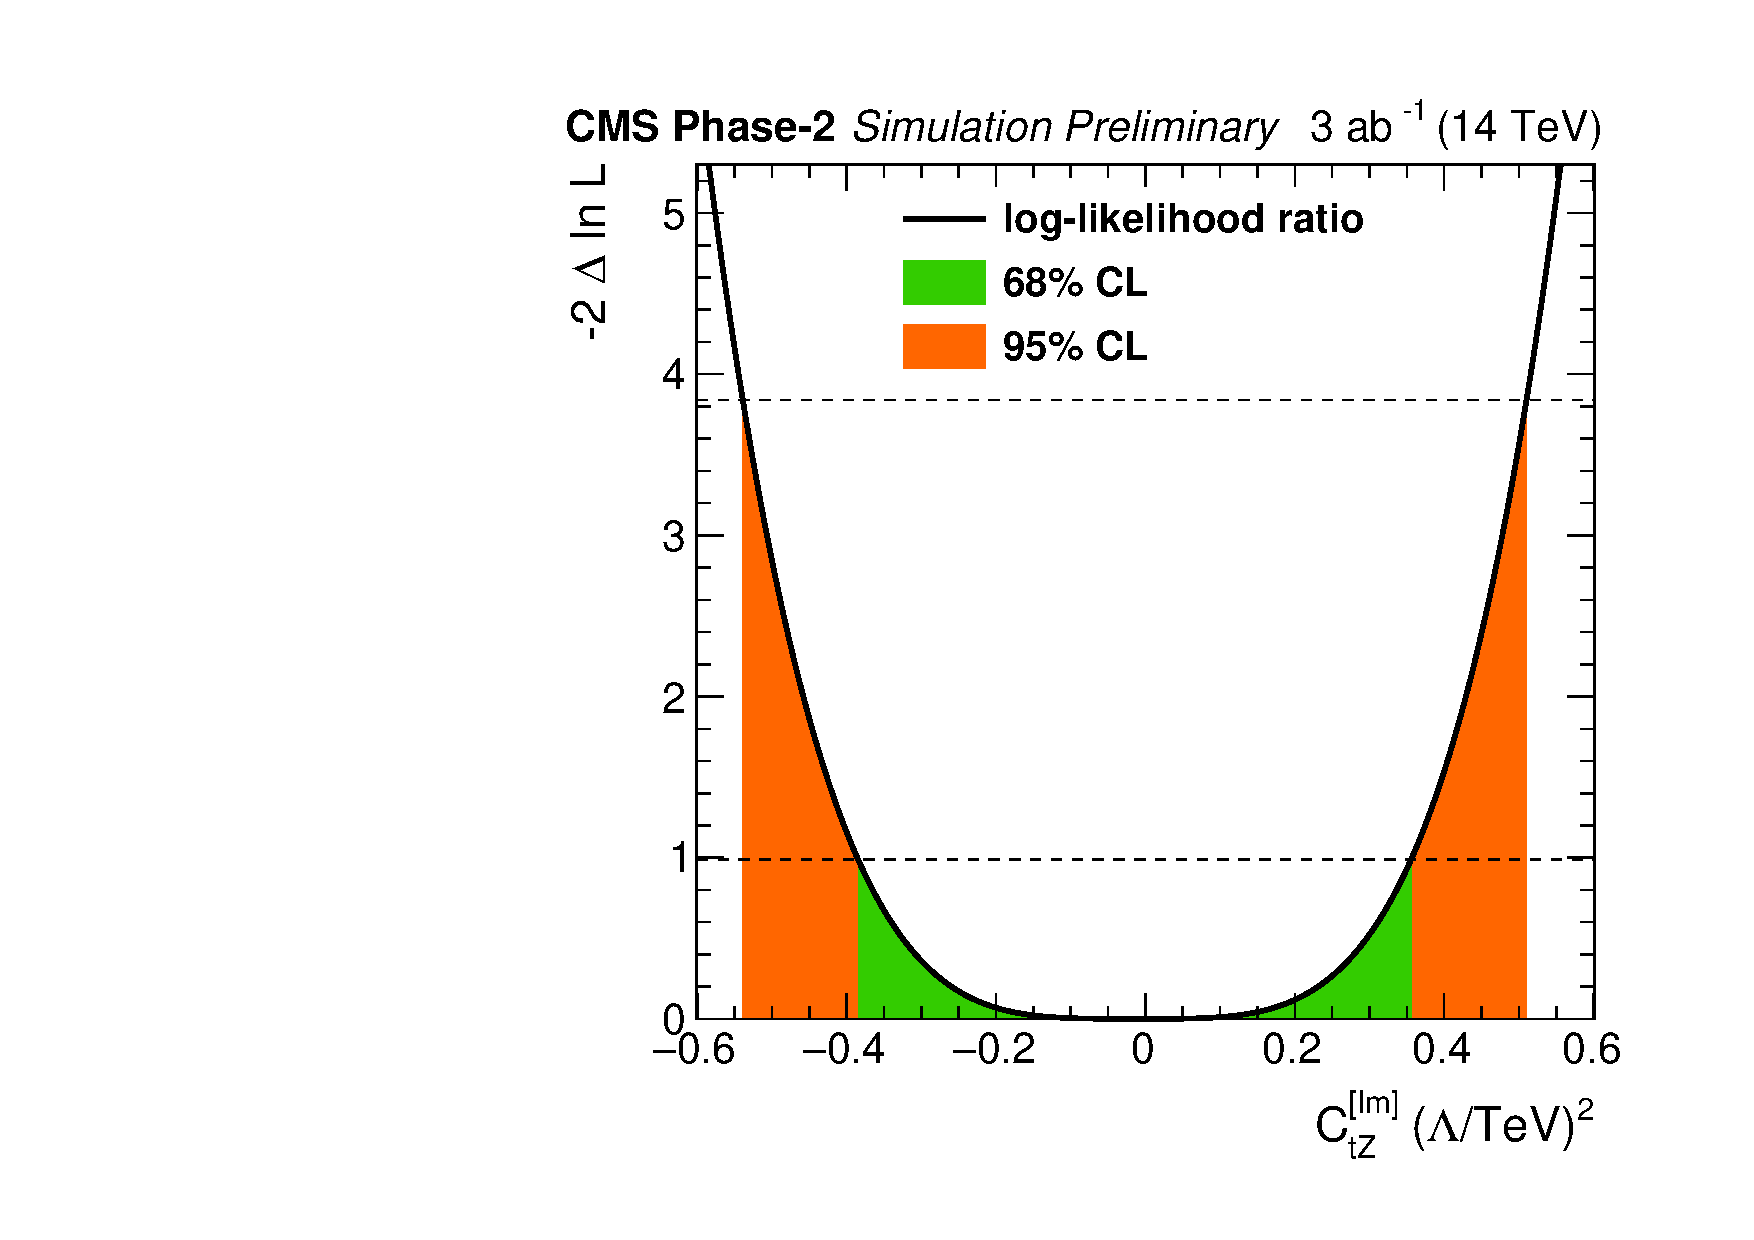
\includegraphics[trim={0.4cm 0.cm 0.8cm 0.cm},clip,width=0.45\textwidth]{Figures/1D_ctZI_lumi3000_14TeV_CMScombine_r1_fullUnc.pdf}
  \caption{Individual likelihood ratio for the Wilson coefficients cpt and cpQM (top) and ctZ and ctZI (bottom) for the ttZ process.
           Here, only one Wilson coefficient at a time is considered non-zero.
           The 68\% (95\%) CL intervals are given in green (red).
           }
  \label{fig:ttZ_1Dnll}
\end{figure}

\begin{figure}[tbp]
  \centering
    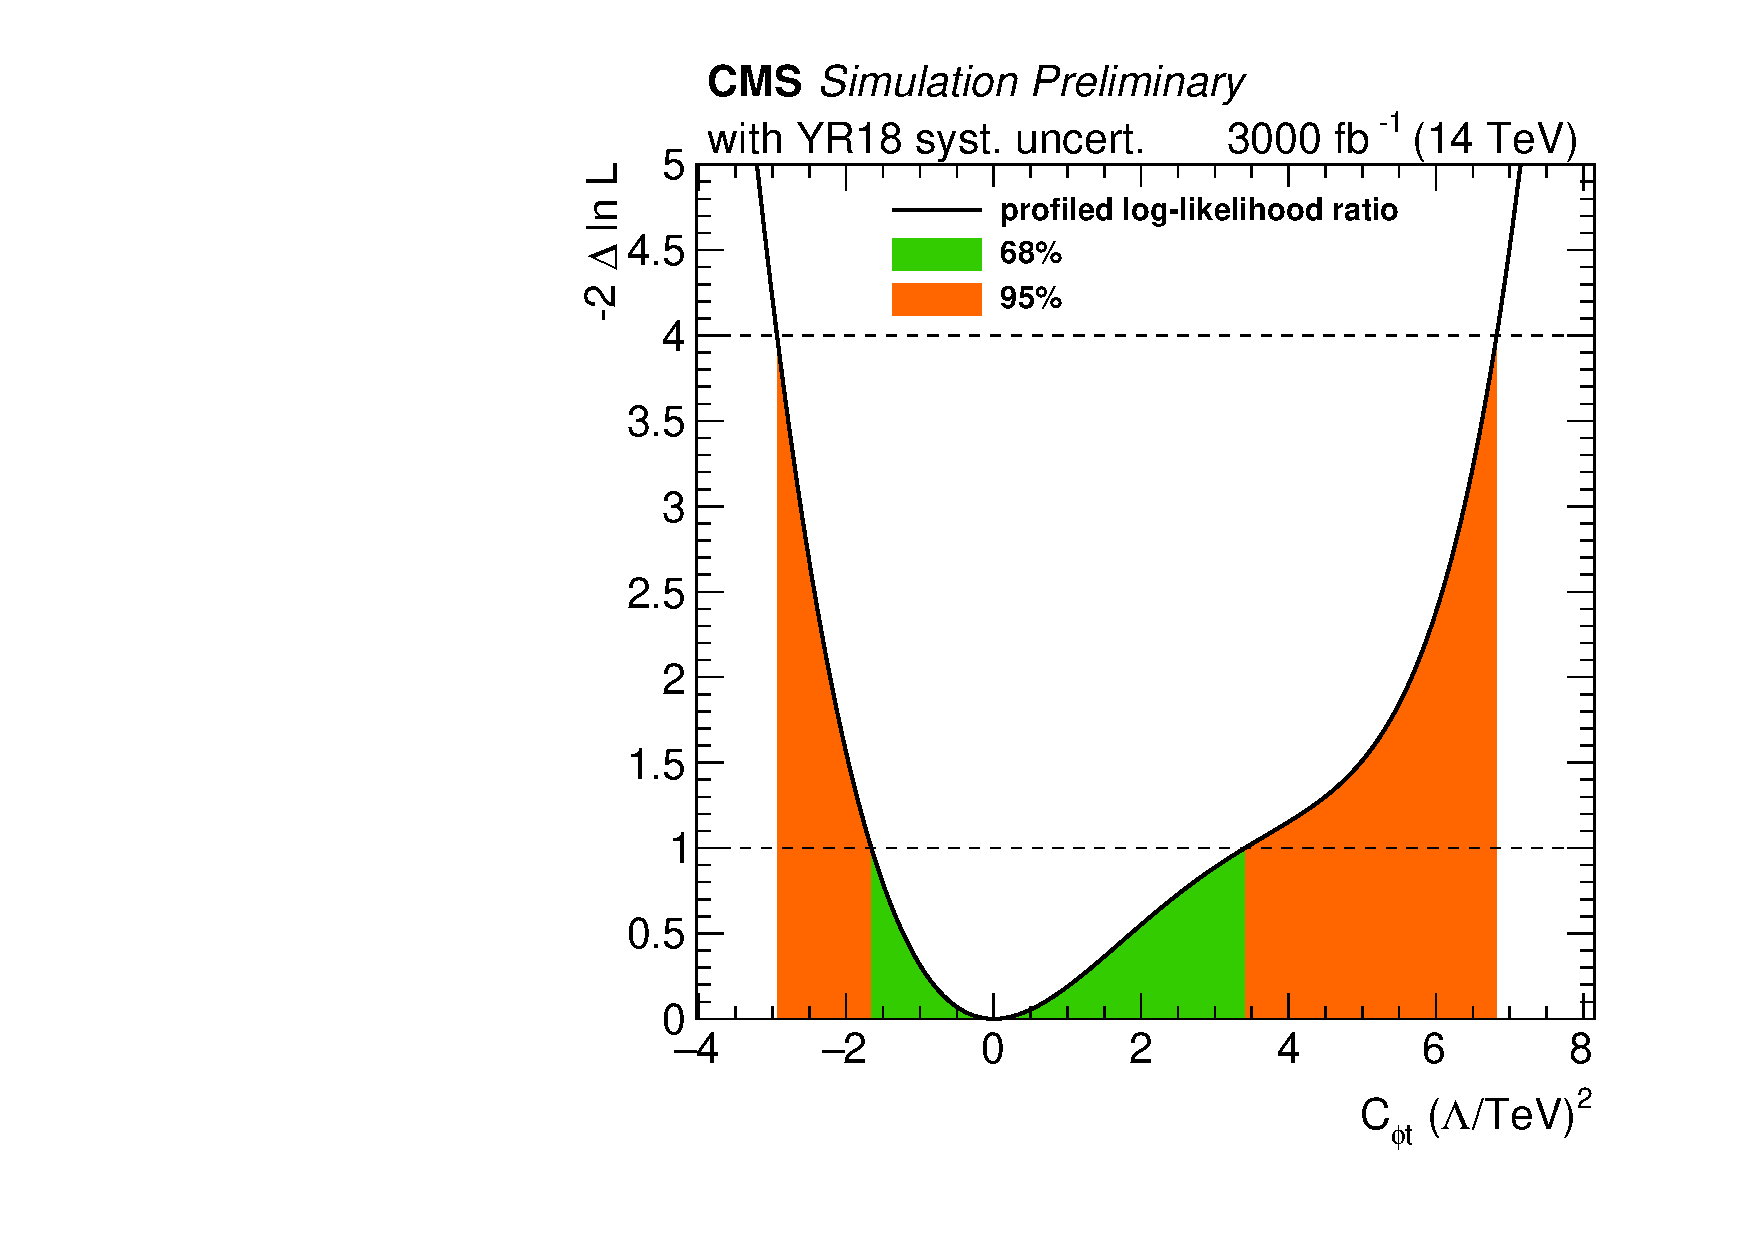
\includegraphics[trim={0.4cm 0.cm 0.8cm 0.cm},clip,width=0.45\textwidth]{Figures/cpt_lumi3000_14TeV_CMScombine_r1_fullUnc.pdf}
    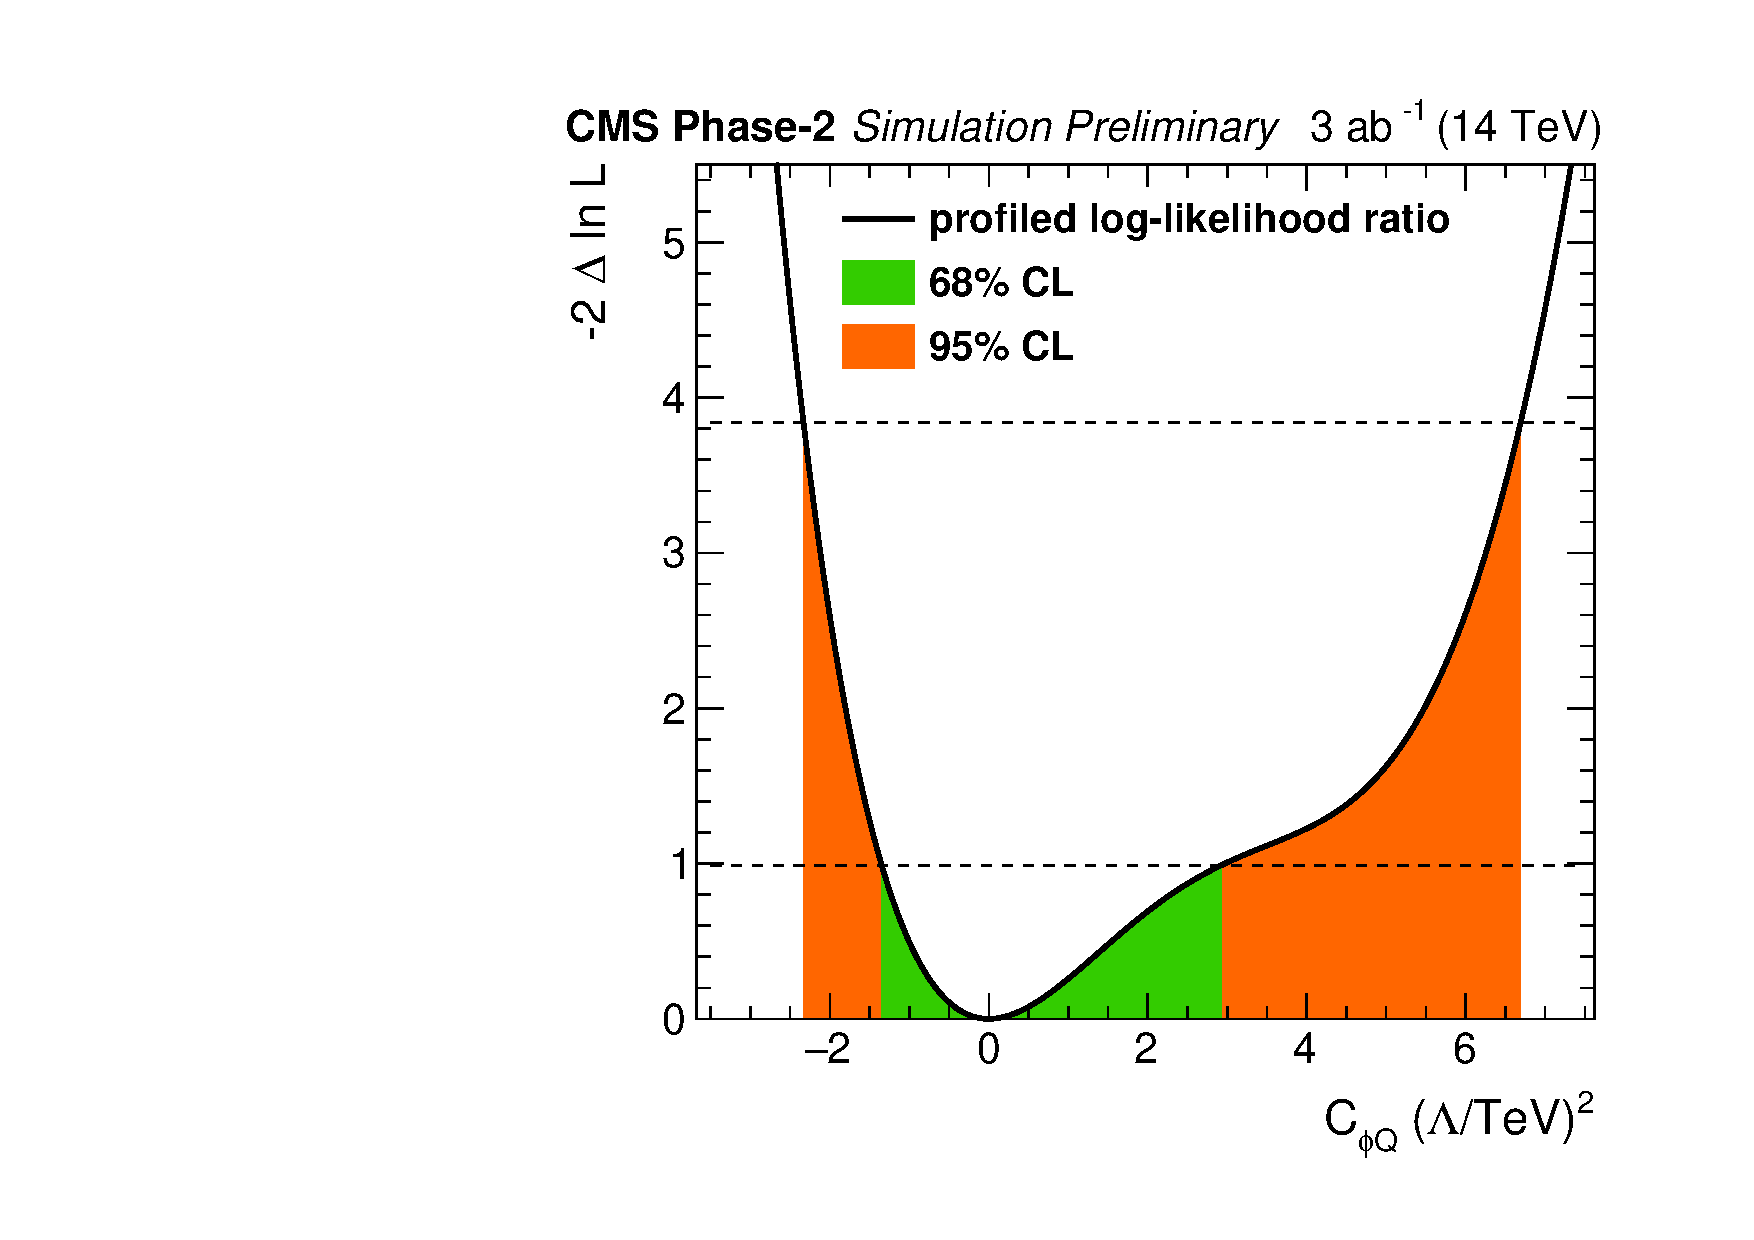
\includegraphics[trim={0.4cm 0.cm 0.8cm 0.cm},clip,width=0.45\textwidth]{Figures/cpQM_lumi3000_14TeV_CMScombine_r1_fullUnc.pdf}
    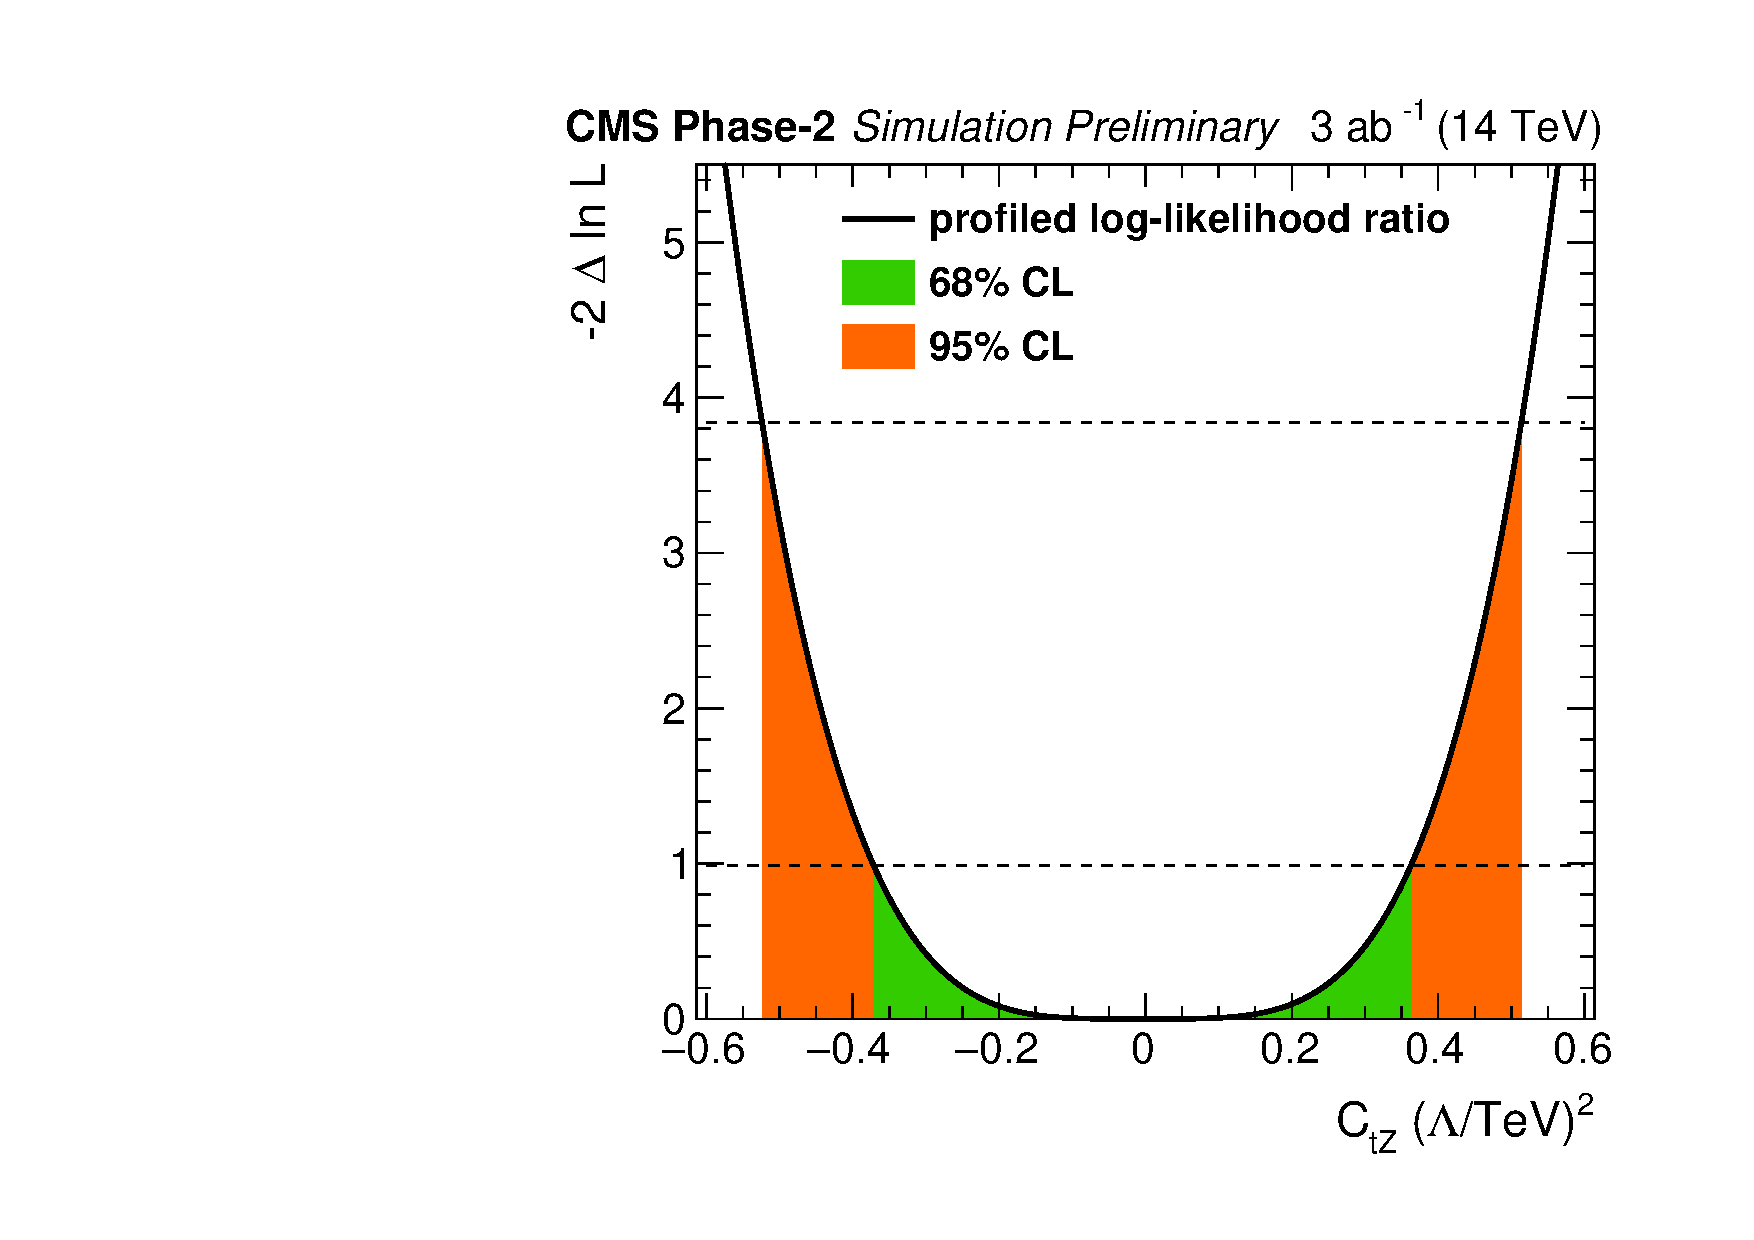
\includegraphics[trim={0.4cm 0.cm 0.8cm 0.cm},clip,width=0.45\textwidth]{Figures/ctZ_lumi3000_14TeV_CMScombine_r1_fullUnc.pdf}
    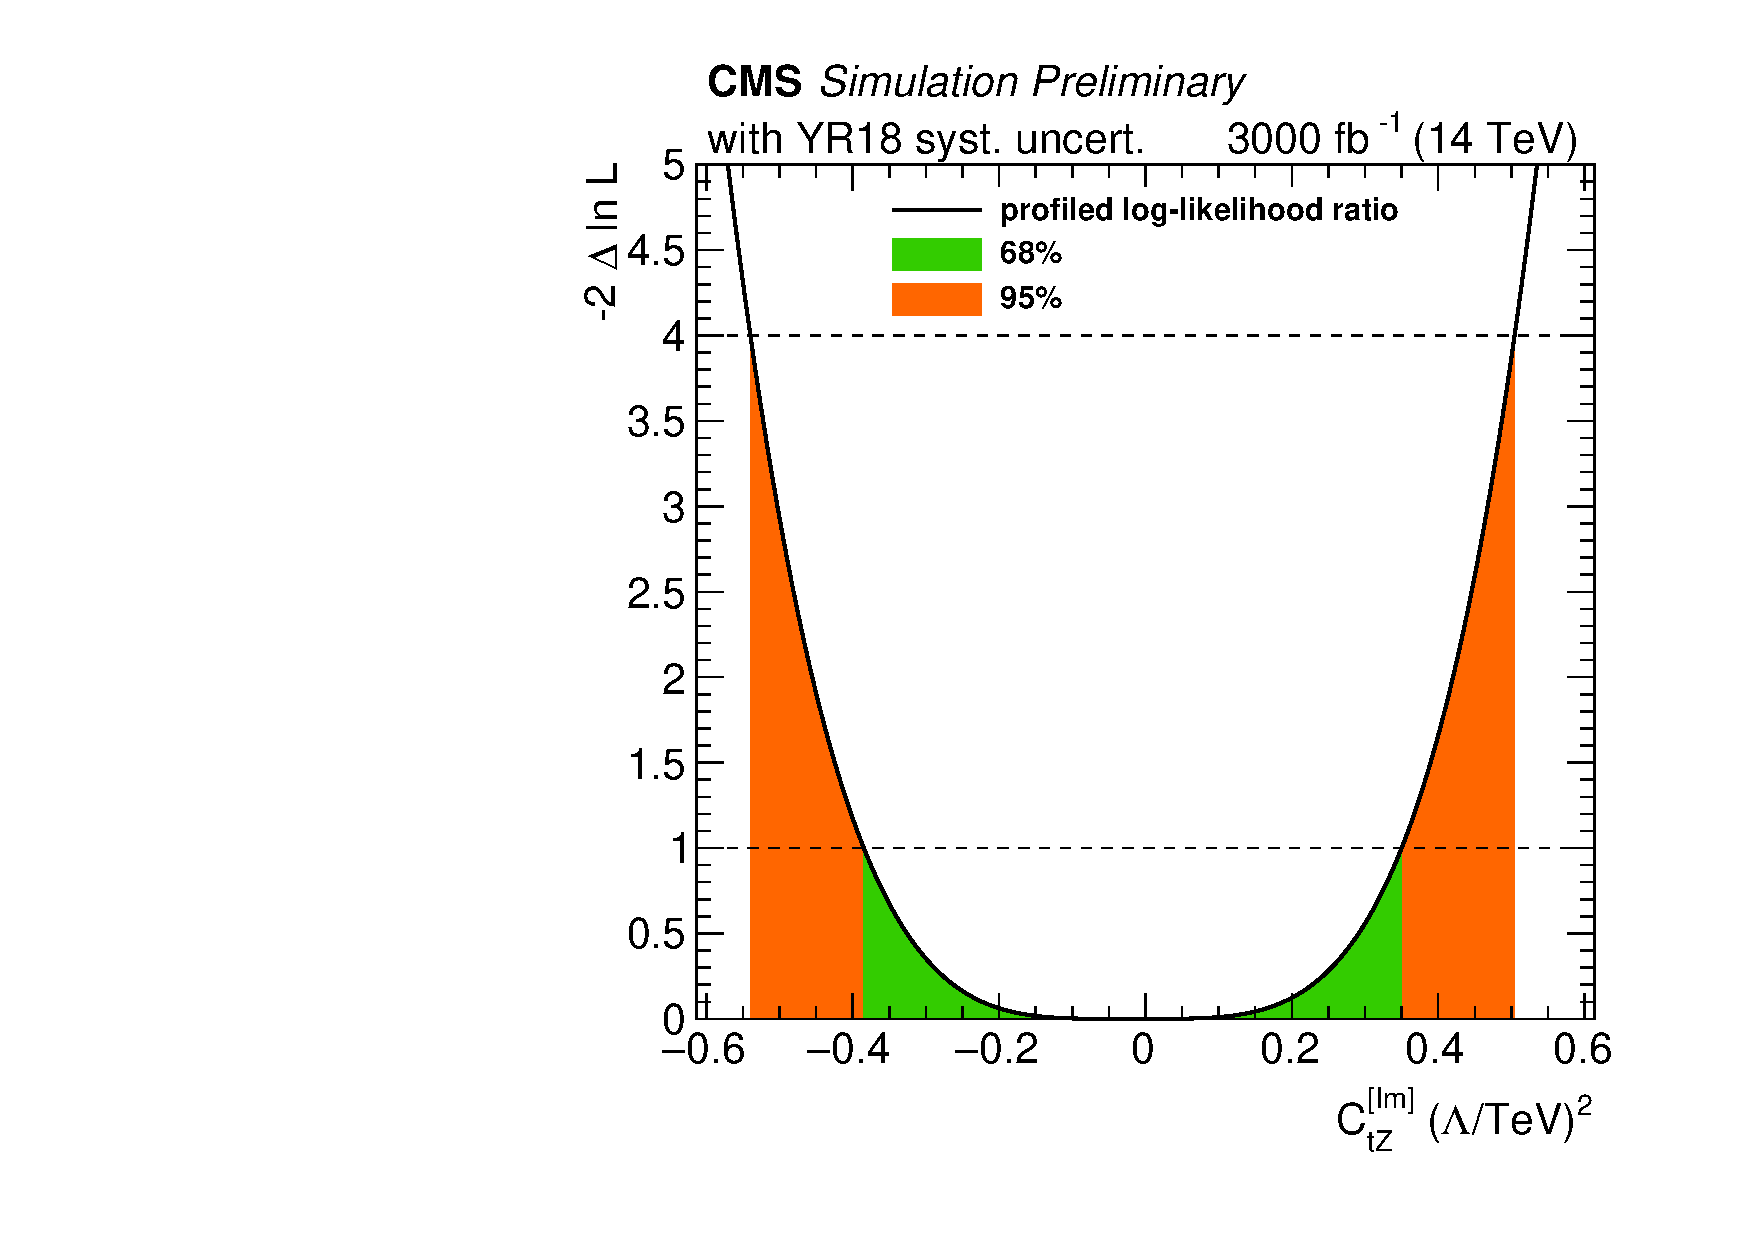
\includegraphics[trim={0.4cm 0.cm 0.8cm 0.cm},clip,width=0.45\textwidth]{Figures/ctZI_lumi3000_14TeV_CMScombine_r1_fullUnc.pdf}
  \caption{Individual profiled likelihood ratio for the Wilson coefficients \cpt and \cpQM (top) and \ctZ and \ctZI (bottom) for the \ttZ process under the SM hypothesis.
           The 68\% (95\%) CL intervals are given in green (red).
           }
  \label{fig:ttZ_1Dprofnll}
\end{figure}

\begin{figure}[tbp]
  \centering
    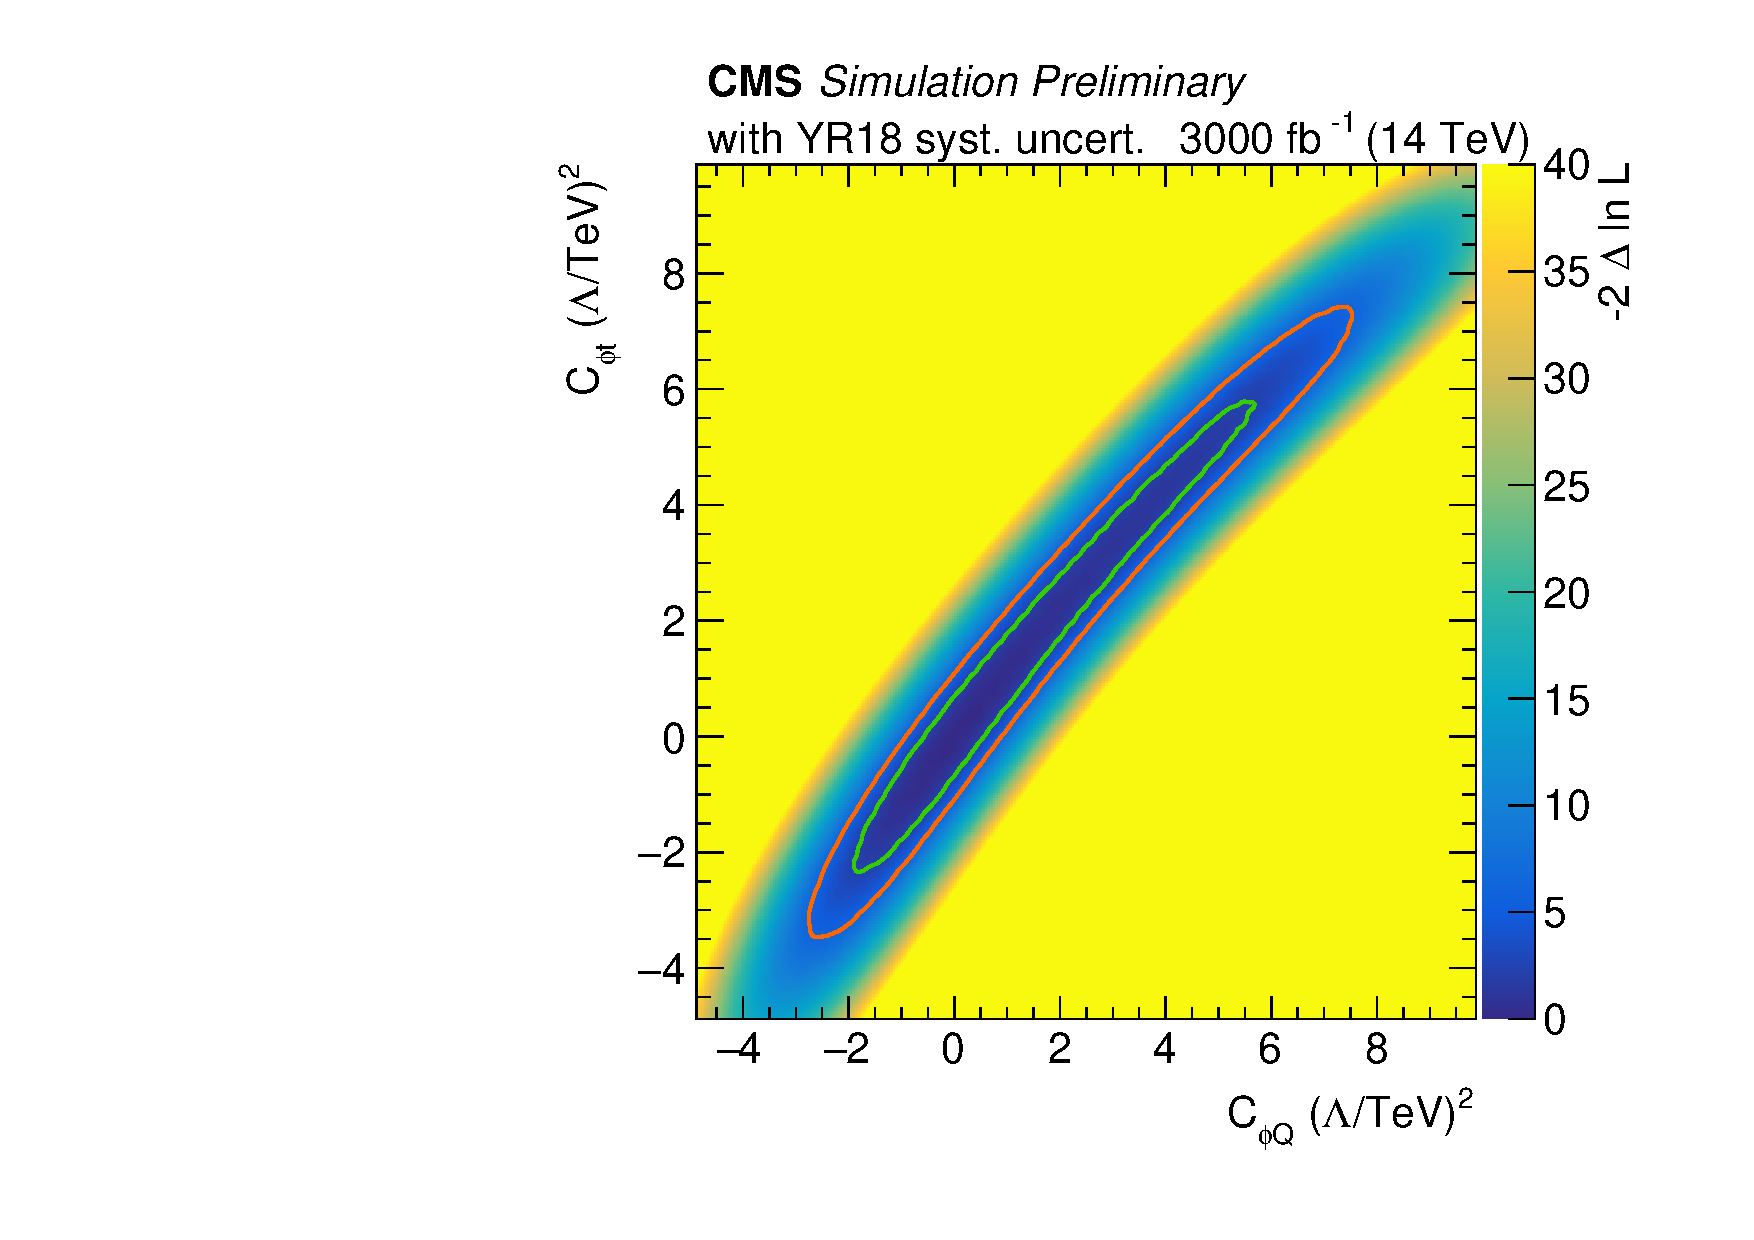
\includegraphics[trim={0.4cm 0.cm 0.8cm 0.cm},clip,width=0.45\textwidth]{Figures/cpQM_cpt_lumi3000_14TeV_CMScombine_r1_fullUnc.pdf}
    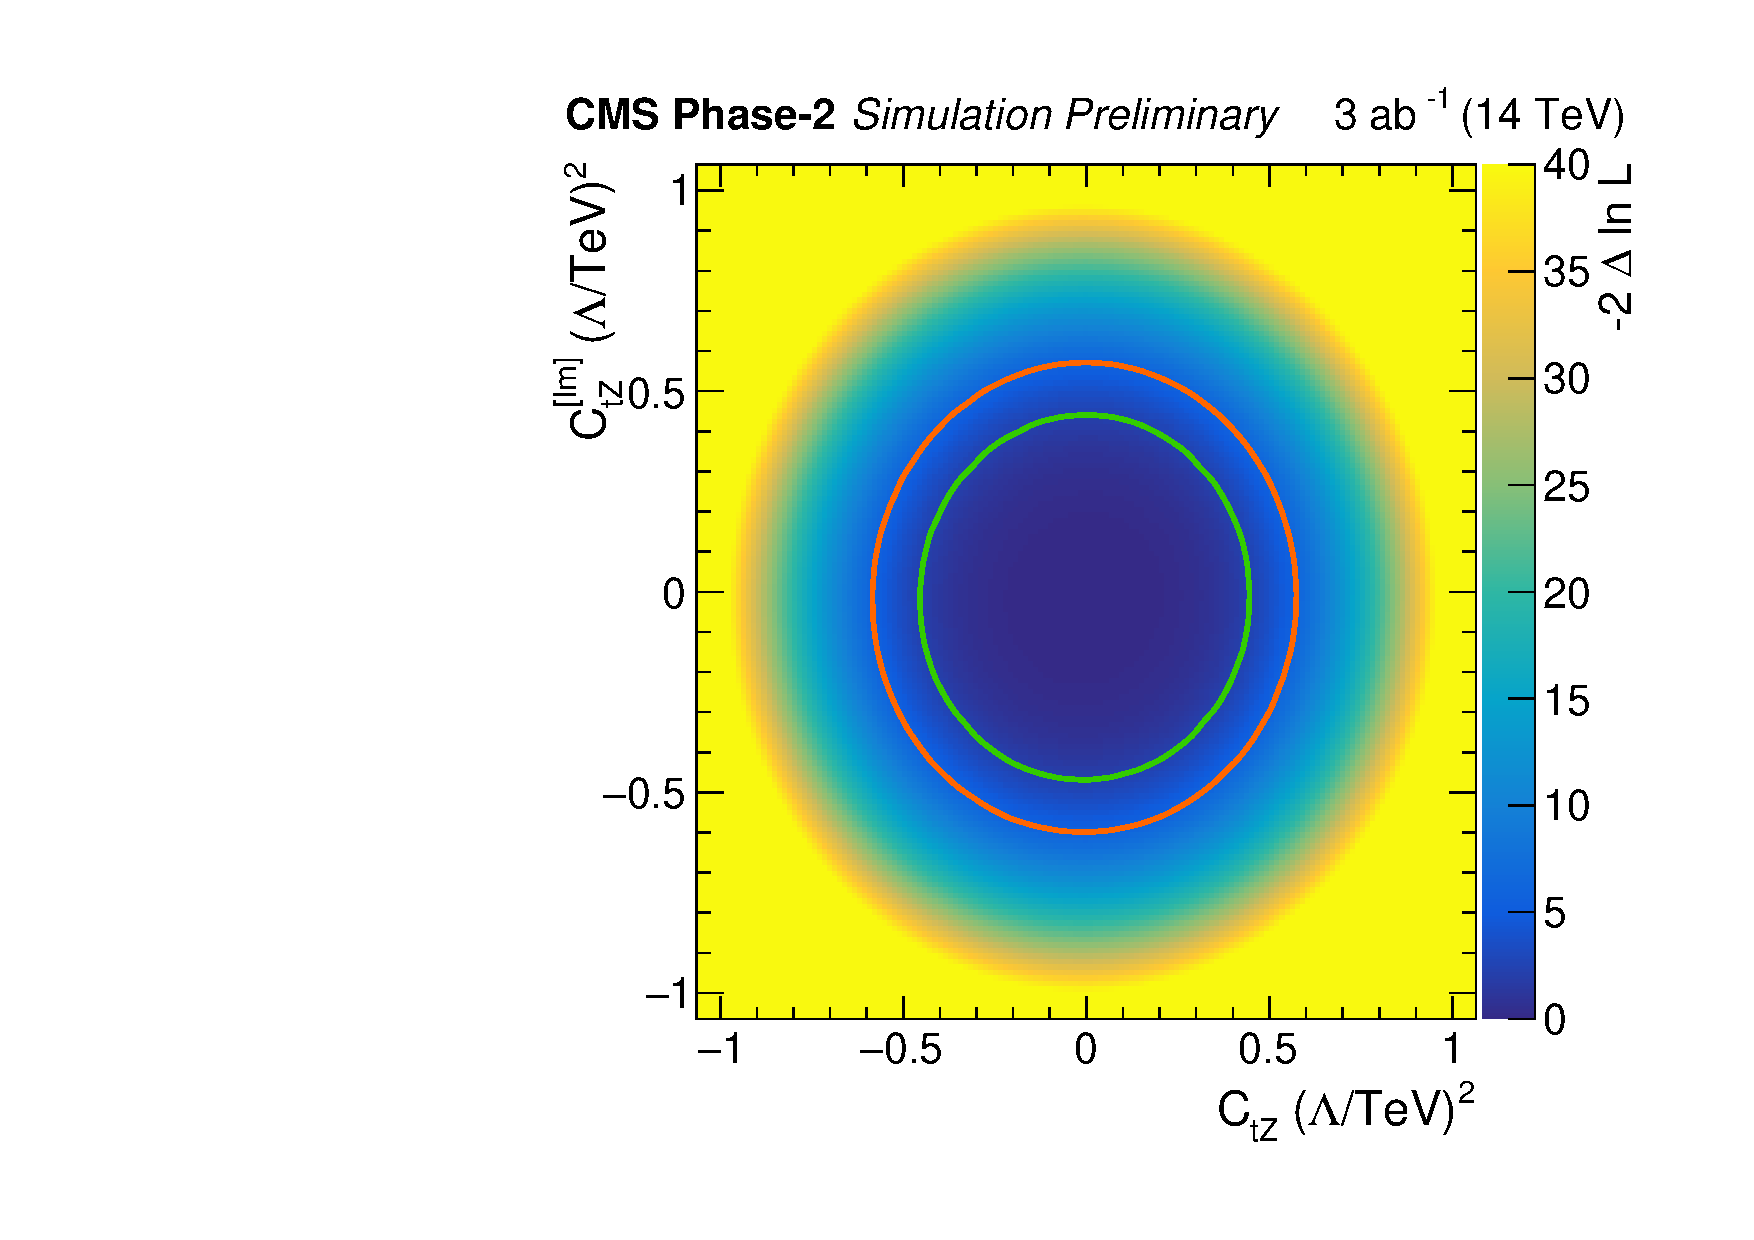
\includegraphics[trim={0.4cm 0.cm 0.8cm 0.cm},clip,width=0.45\textwidth]{Figures/ctZ_ctZI_lumi3000_14TeV_CMScombine_r1_fullUnc.pdf}
  \caption{Scan of the negative likelihood in the \cpQM/\cpt (left) and \ctZ/\ctZI parameter planes (right) for the \ttZ process under the SM hypothesis.
           The 68\% (95\%) CL contour lines are given in green (red).
           }
  \label{fig:ttZ_nll}
\end{figure}

\clearpage
\bibliographystyle{unsrt}
\bibliography{FTR-18-036-summary.bib}

\end{document}
